\section{Part 1: Extracting the P300 Response}

\begin{taskbox}[Part 1: introduction in the lab manual]
The EEG signal (\texttt{ERP\_EEG}) stored in \texttt{EEG\_ERP.mat} contains EEG recorded from one channel (Pz). The brain signal was recorded in response to a visual stimulus and contains the P300 event-related potential and background EEG. 2550 trials were performed and the brain signal was recorded in response to the stimulus. The sampling frequency is 240 Hz, and in each trial the signal was recorded from the stimulus onset until 1 second after it. Assuming that the latency of the brain response to the stimulus is the same in all trials, we want to use synchronous averaging to determine the minimum number of trials needed to extract the P300 response.
\end{taskbox}

\subsection*{Data and synchronous averaging}

The data of the first part consist of 2550 one-second repetitions of channel Pz with a sampling frequency of 240~Hz. Each column of the matrix \texttt{ERP\_EEG} represents one repetition and each row one time sample. The time axis therefore extends from zero to 995.83~ms. To extract the event-related response, we used synchronous averaging, as in the lab notes. Assuming that the response time is the same across repetitions, the stimulus-related component remains in the average, and the unrelated background EEG components are reduced to some extent. This process does not increase the true amplitude of P300; it improves the ratio of the constant response to the variable background. No pre-stimulus samples are provided, so no pre-stimulus baseline correction was performed. The unit of amplitude calibration is also not specified in the metadata of the file, and all amplitudes are reported in the original unit of the data.

\subsection*{(a) Waveform change with the number of repetitions}
\begin{taskbox}
For $N=100{:}100{:}2500$, plot the average response obtained from $N$ patterns. Plot the graphs in a single figure and compare them as $N$ increases.
\end{taskbox}

The average response was computed for $N$ equal to 100, 200, up to 2500 and drawn in a single common figure containing 25 curves. For a small number of repetitions, the fluctuation and the amplitude of the wave are larger, and the response shape changes as repetitions are added. As $N$ increases, the overall shape of the average responses converges; the positive peaks a few hundred milliseconds after the stimulus become more stable, and the late variations become smaller. The largest positive peak of the average of all 2550 repetitions, in the descriptive interval of 200 to 600~ms, has an amplitude of 1.6785 and a latency of 283.33~ms. This number was obtained from the data, and the peak time should not be forcibly assumed to be exactly 300~ms.

\begin{figure}[H]
\centering
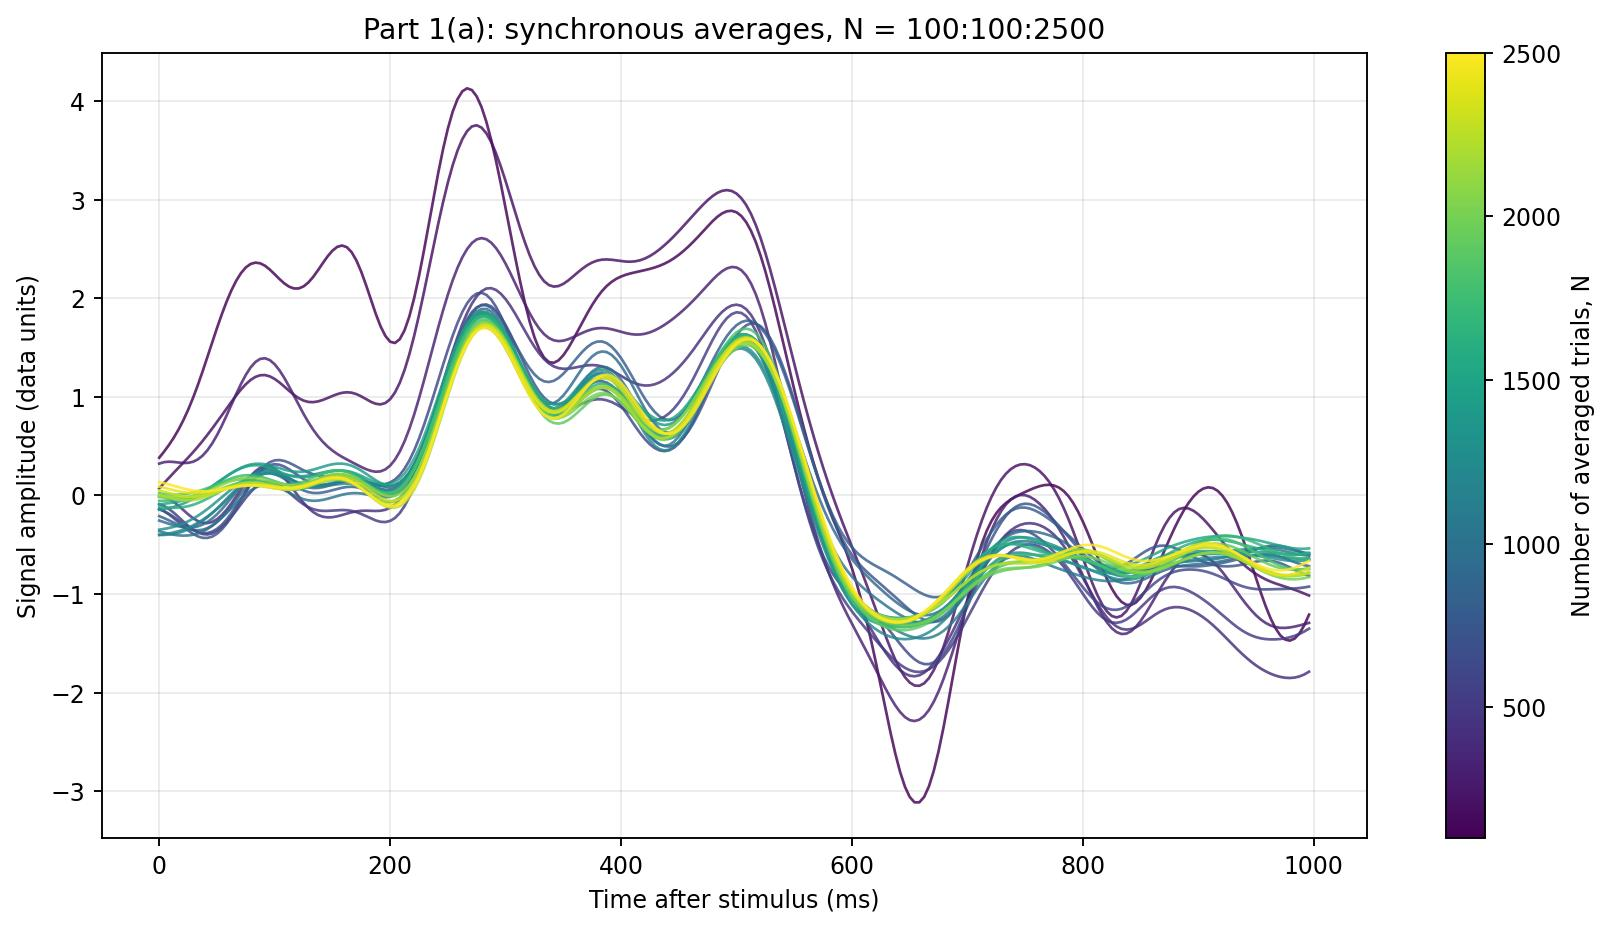
\includegraphics[width=0.95\textwidth]{fig01_p300_averages_n100_to_n2500.png}
\caption{Synchronous average for $N$ from 100 to 2500 in steps of 100; the color of each curve indicates the number of repetitions.}
\label{fig:p300avg}
\end{figure}

\subsection*{(b) and (c) Indices of the change of the average response}
\begin{taskbox}
\textbf{(b)} For $N=1{:}2550$, plot the maximum absolute amplitude of the signal versus the number of averaged patterns in a single graph.\\
\textbf{(c)} Plot the root mean square (RMS) error between the $N$-th average pattern and the $(N-1)$-th average pattern versus the number of averaged patterns $N=1{:}2550$ in a single graph.
\end{taskbox}

\paragraph{(b) Maximum absolute amplitude.} For each number of repetitions, the maximum absolute value of the average response was computed. This value is 10.3790 for one repetition, 4.1276 for 100 repetitions, 2.1013 for 400 repetitions, 1.7106 for 1200 repetitions, and 1.6785 for 2550 repetitions. The overall trend is decreasing, but adding one repetition can cause a local increase or decrease.
\begin{equation}
A_N=\max_k\,|M_N[k]|
\end{equation}

\begin{figure}[H]
\centering
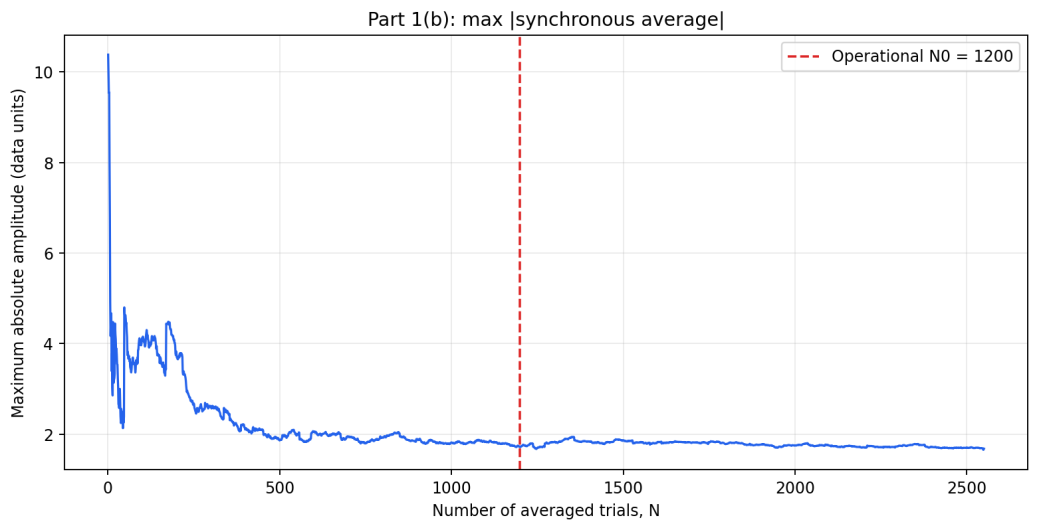
\includegraphics[width=0.85\textwidth]{fig02_max_abs_amplitude_vs_n.png}
\caption{Maximum absolute value of the average response versus the number of repetitions.}
\label{fig:maxabs}
\end{figure}

\paragraph{(c) Differences of successive averages.} The root mean square of the difference between two successive average responses was computed. For $N$ equal to one this quantity is not defined, and it was stored as NaN. Its values at 100, 400 and 1200 repetitions are 0.14025, 0.02364 and 0.00588, respectively. The decreasing trend is consistent with stability; nevertheless, the difference between averages is inherently divided by $N$, and its becoming small does not by itself prove the detection of P300.
\begin{equation}
E_N=\mathrm{RMS}\!\left(M_N-M_{N-1}\right);\qquad N\ge 2
\end{equation}

\begin{figure}[H]
\centering
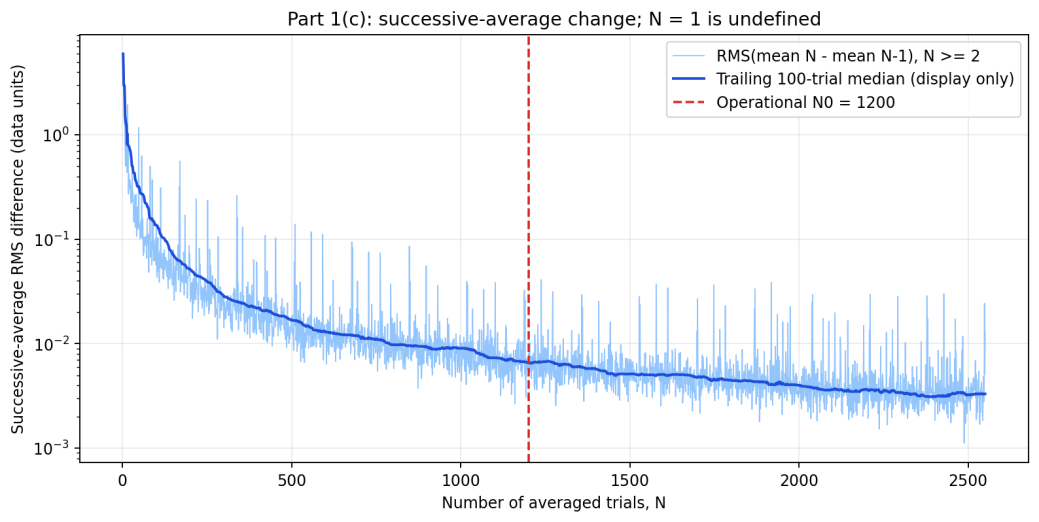
\includegraphics[width=0.85\textwidth]{fig03_rms_difference_consecutive_averages.png}
\caption{RMS difference of successive averages; the vertical axis is logarithmic and the value $N=1$ is undefined.}
\label{fig:rmsdiff}
\end{figure}

\subsection*{(d) Determining the selected number of repetitions}
\begin{taskbox}
Using the results obtained in parts (a), (b) and (c), what is the required number of trials from which the P300 response can be extracted? (Call the obtained number $N_0$.)
\end{taskbox}

The exercise statement did not set a specific numerical threshold for the appearance of the response; we therefore determined the required number of repetitions with an operational criterion for waveform stability. The responses were checked at intervals of 100 repetitions. At each checkpoint, two conditions were required. First, the range of variation of the maximum absolute amplitude of the response in the last 100 repetitions, relative to the median of the same quantity in that interval, is at most 10 percent. Second, the median of the RMS difference of successive averages in the same interval, relative to the maximum absolute response at the checkpoint, is at most one percent. After both conditions held simultaneously at three consecutive checkpoints, the number 1200 repetitions was chosen, and its waveform was also compared with the responses obtained from larger numbers.

This number is neither a unique physiological minimum nor a significance test. For example, by lowering the amplitude-fluctuation threshold to 5 percent, $N_0$ reaches 1900; with a threshold of 15 percent, keeping the one-percent RMS limit, the value 700 is obtained. The number 1200 must therefore be reported together with the definition of the criterion.

\begin{figure}[H]
\centering
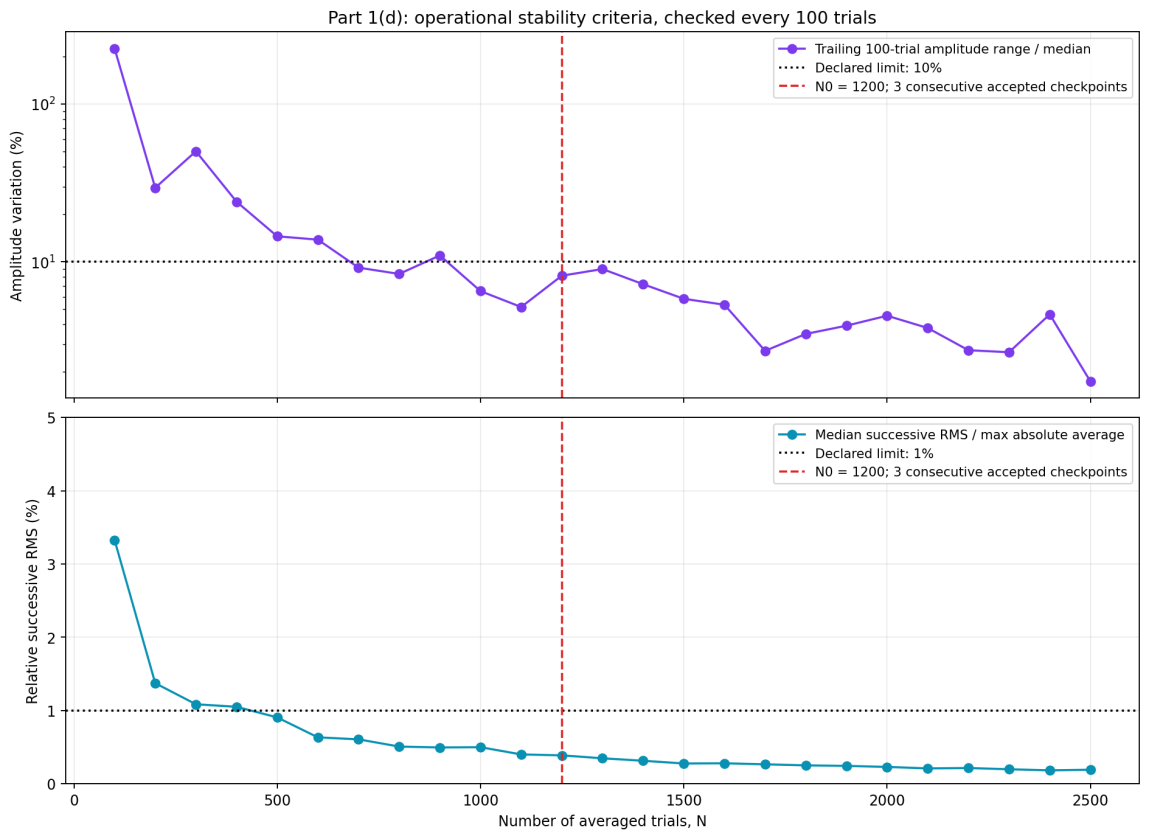
\includegraphics[width=0.85\textwidth]{fig04_stability_criteria_n0.png}
\caption{The two stability criteria and the confirmation point of three consecutive checks at $N_0=1200$.}
\label{fig:stability}
\end{figure}

\begin{table}[H]
\centering
\caption{Sensitivity of the selected number to the amplitude stability threshold, with three consecutive checks held fixed.}
\begin{tabular}{@{}ccc@{}}
\toprule
\textbf{Amplitude-change threshold} & \textbf{Relative RMS threshold} & $N_0$\\
\midrule
5\%  & 1\% & 1900\\
10\% & 1\% & 1200\\
15\% & 1\% & 700\\
\bottomrule
\end{tabular}
\end{table}

\subsection*{(e) Comparison of the number of repetitions and the way of selection}
\begin{taskbox}
In a single graph, plot the average response obtained in part (d) together with the following average responses, and compare them. Examine and analyze the obtained results: the average response for $N=2550$; for $N=N_0/3$; for $N=N_0$ with $N_0$ randomly chosen responses out of the 2550 responses; and for $N=N_0/3$ with $N_0/3$ randomly chosen responses out of the 2550 responses.
\end{taskbox}

The average of the first 1200 repetitions was compared with the average of all 2550 repetitions, the first 400 repetitions, 1200 random repetitions and 400 random repetitions. The random selections were made with seed 42 and without replacement. For the descriptive comparison, the average of all repetitions was taken as the reference.

\begin{figure}[H]
\centering
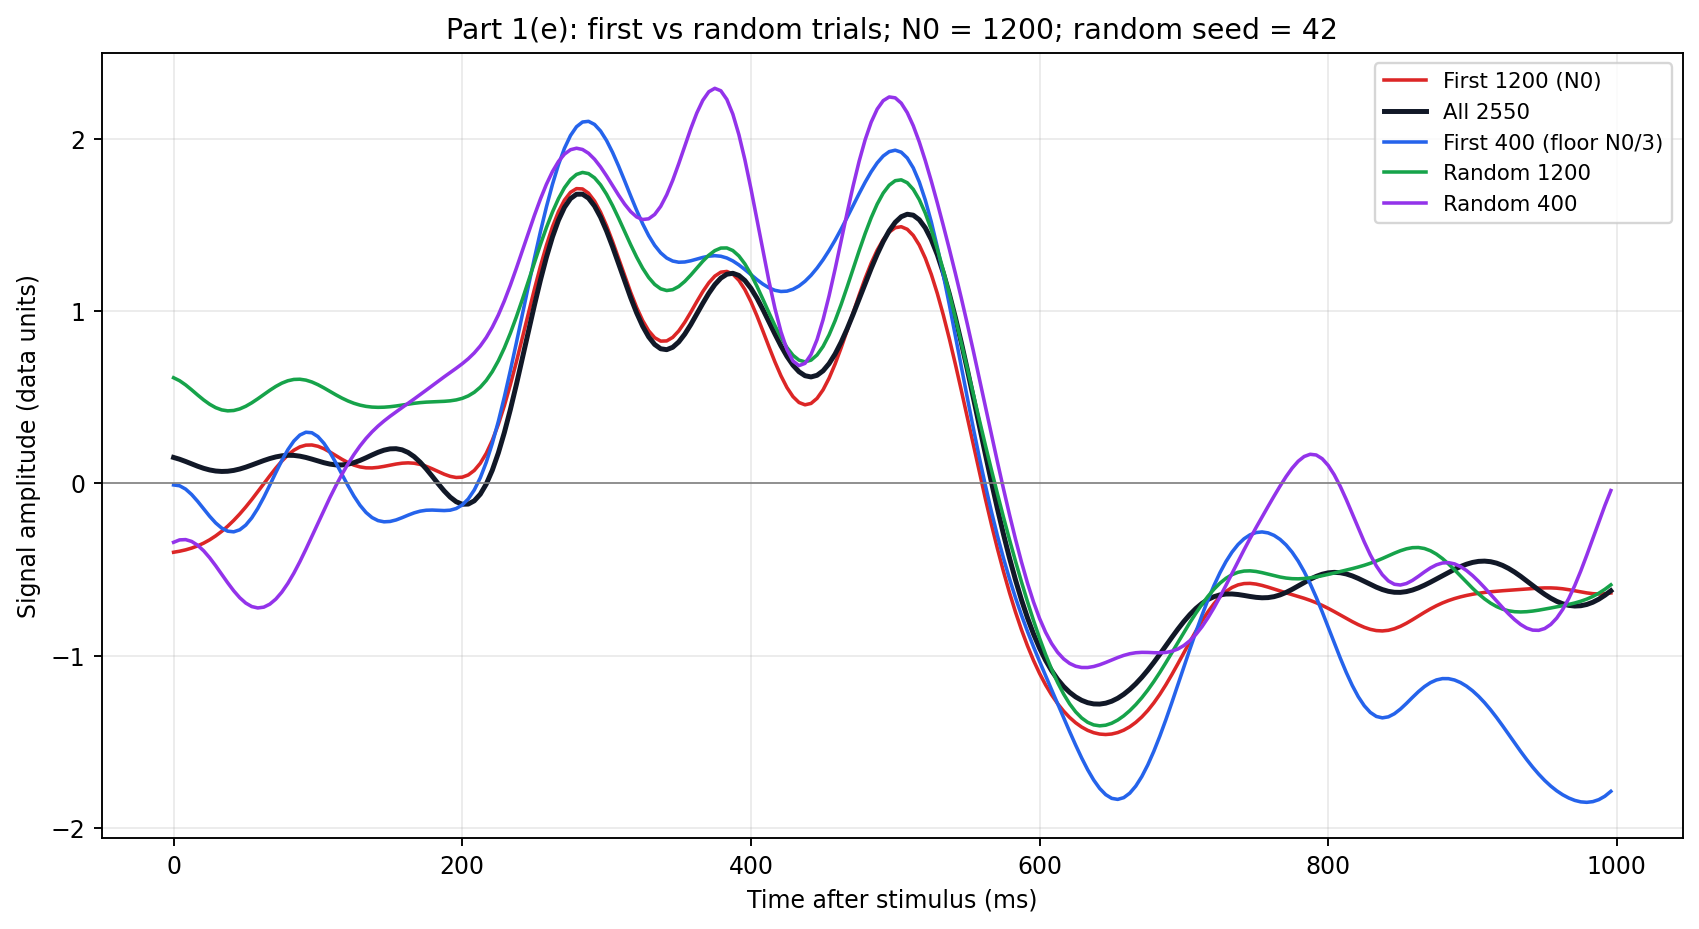
\includegraphics[width=0.85\textwidth]{fig05_comparison_of_five_averages.png}
\caption{Comparison of the five requested responses; the average of all 2550 repetitions is marked with a black line.}
\label{fig:fiveavg}
\end{figure}

\begin{table}[H]
\centering
\caption{Descriptive indices relative to the average of all repetitions; the positive peak is reported in the interval 200 to 600~ms.}
\begin{tabular}{@{}lcccc@{}}
\toprule
\textbf{Response} & \textbf{Positive peak} & \textbf{Latency (ms)} & \textbf{RMS difference} & \textbf{Correlation}\\
\midrule
First 1200 & 1.7106 & 279.17 & 0.1660 & 0.9872\\
All 2550   & 1.6785 & 283.33 & 0.0000 & 1.0000\\
First 400  & 2.1013 & 287.50 & 0.4924 & 0.9551\\
Random 1200 & 1.8046 & 283.33 & 0.2534 & 0.9802\\
Random 400 & 2.2928 & 375.00 & 0.4980 & 0.9193\\
\bottomrule
\end{tabular}
\end{table}

With this specific selection, both 1200-repetition averages are closer to the overall reference than the 400-repetition averages. Random selection has not necessarily made the result better; in this same run, the first 1200 repetitions are closer to the reference than the random sample of 1200 repetitions. The result of one sampling cannot be generalized to all random selections. Moreover, the overall reference itself contains noise and includes the compared repetitions; these indices therefore do not constitute an independent validation.

\subsection*{(f) The number of repetitions in real P300 applications}
\begin{taskbox}
Investigate a few real experiments based on the P300 signal. In real experiments that use P300 patterns (such as P300-based brain-computer interfaces), how many repetitions of the P300 pattern are used? Is this number consistent with the results obtained in the previous parts? Explain the reason for this difference.
\end{taskbox}

In applied studies, a ``repetition'' may refer to the number of sequences, the number of stimulus flashes, or the number of target events. In a $6\times6$ row-column keyboard, one sequence consists of 12 flashes, and the target letter is flashed twice, once with its row and once with its column. Fifteen sequences are therefore equivalent to 180 flashes in total and 30 target events. This unit differs from each single-event column of the file of this exercise.

Lu et al.\ in 2013 used 15 complete sequences for each letter. In the study of Nijboer et al.\ in 2008, the first phase consisted of 20 sequences for each letter, and in the second phase the number of sequences for four participants was chosen as 14, 13, 7 and 4, respectively. Townsend et al.\ in 2010 used five sequences in calibration and adjusted the number of sequences of the online test for each person. The numbers in these examples are usually smaller than $N_0$ of this exercise, but the aim of a practical system is target selection with multichannel features and a trained classifier; this exercise examines the stability of the waveform of a single channel with averaging. The difference in the unit of repetition, the amount of noise, the person's attention, the timing of the stimuli and the success criterion limits a direct comparison of the numbers. No universal minimum for the required number can be derived from these papers.

\begin{table}[H]
\centering
\caption{Applied examples; the number of sequences is not the same as the number of single-event responses of the exercise.}
\begin{tabularx}{\textwidth}{@{}>{\raggedright\arraybackslash}p{3.1cm}>{\raggedright\arraybackslash}X>{\raggedright\arraybackslash}X@{}}
\toprule
\textbf{Study} & \textbf{Sequence protocol} & \textbf{Target events}\\
\midrule
Lu et al.\ 2013 & 15 sequences of 12 stimuli per letter & 30 target events; 180 flashes in total\\
Nijboer et al.\ 2008 & 20 sequences in the first phase; 4 to 14 in the second phase & 40 target events in the first phase\\
Townsend et al.\ 2010 & 5 calibration sequences; individual adjustment in the test & 10 target events in calibration\\
\bottomrule
\end{tabularx}
\end{table}

This difference does not prove an inconsistency between the result of the exercise and practical application. To reveal a stable waveform, a criterion different from that of selecting one letter correctly with a multichannel classifier was used. The appropriate number of repetitions must be reported together with the counting unit, the recording conditions and the decision criterion.
